\section{Results}
\label{sec:results}

All quantitative results below reconstruct from the canonical combined synthesis and the underlying HIGH/LOW/UNSEEN analysis artifacts.
No numbers were re-estimated for this manuscript.
Where we round to two decimal places in percentage points, rounding follows the combined evidence tables and does not change sign or qualitative interpretation.

\subsection{Integrity and validity}
HIGH and UNSEEN each collected and evaluated 42/42 planned runs with seven valid paired configurations (21 pairs).
LOW collected 42/42 retained runs but has six valid paired configurations (18 pairs) because the Qwen cell is \texttt{INVALID --- MODEL MISMATCH} (\Cref{sec:repro}).
Integrity gates (unique run IDs; complete Direct$\leftrightarrow$Primed pairing structure) pass on all three regimes.
These integrity facts are prerequisites for interpreting any mean $\Delta$: a missing or mismatched pair would silently break the Direct/Primed contrast.

\subsection{Central configuration-level $\Delta$ table}
\Cref{tab:deltas} is the primary quantitative table for later discussion and for RQ1--RQ4.
Reading the table by columns emphasizes regime behaviour; reading by rows emphasizes configuration heterogeneity.
Both views are necessary.
A column-only summary would hide Gemini's HIGH negatives; a row-only focus on one ``successful'' configuration would hide attenuation and invalid cells elsewhere.

\begin{table}[t]
\centering
\caption{Central cross-regime configuration mean $\Delta$ (canonical coverage, percentage points).
LOW Qwen cell is invalid and shown as ---.}
\label{tab:deltas}
\begin{tabular}{@{}lrrr@{}}
\toprule
\textbf{Configuration} & \textbf{HIGH $\Delta$} & \textbf{LOW $\Delta$} & \textbf{UNSEEN $\Delta$} \\
\midrule
Gemini ON & $-0.55$ & $+13.23$ & $+5.68$ \\
Gemini OFF & $-1.75$ & $+10.40$ & $+6.09$ \\
Claude Sonnet 5 & $+14.28$ & $+12.11$ & $+6.42$ \\
DeepSeek Expert ON & $+9.25$ & $+6.19$ & $+3.83$ \\
Qwen 3.8 Max Fast & $+5.18$ & --- & $+3.52$ \\
GPT-5.6 Luna & $+8.62$ & $+5.31$ & $+5.52$ \\
Grok 4.5 Fast & $+14.49$ & $+3.95$ & $+7.12$ \\
\bottomrule
\end{tabular}
\begin{flushleft}
\footnotesize
Source: \texttt{experiments/exp004-modelscreen/phase2b/analysis/combined/cross\_regime\_table.csv}.
Each cell is the mean of three replicate $\Delta_i$ values except LOW Qwen (invalid model mismatch).
\end{flushleft}
\end{table}


\subsection{Direct and Primed means}
In addition to $\Delta$, \Cref{tab:dpmeans} reports configuration-level Direct and Primed mean coverage.
This table clarifies whether a positive $\Delta$ arises from a large Primed gain, a low Direct baseline, or both.
For example, Gemini LOW combines comparatively low Direct means with substantially higher Primed means, whereas several HIGH positives combine mid Direct means with Primed means above 80\%.
Absolute Direct/Primed levels should be read separately from $\Delta$: a large positive $\Delta$ can arise from a low Direct baseline, a high Primed ceiling, or both, and absolute coverage remains a screening metric rather than a quality score.
\begin{table}[t]
\centering
\caption{Direct and Primed mean canonical coverage (\%) by configuration and regime.
LOW Qwen paired means are omitted (invalid).}
\label{tab:dpmeans}
\scriptsize
\begin{tabular}{@{}lrrrrrr@{}}
\toprule
 & \multicolumn{2}{c}{\textbf{HIGH}} & \multicolumn{2}{c}{\textbf{LOW}} & \multicolumn{2}{c}{\textbf{UNSEEN}} \\
\cmidrule(lr){2-3}\cmidrule(lr){4-5}\cmidrule(lr){6-7}
\textbf{Config.} & D & P & D & P & D & P \\
\midrule
Gemini ON & 68.68 & 68.13 & 64.33 & 77.56 & 65.77 & 71.45 \\
Gemini OFF & 67.20 & 65.45 & 64.51 & 74.91 & 63.85 & 69.95 \\
Claude & 69.29 & 83.57 & 65.72 & 77.83 & 66.07 & 72.48 \\
DeepSeek & 74.53 & 83.78 & 68.93 & 75.12 & 67.97 & 71.80 \\
Qwen & 76.36 & 81.54 & --- & --- & 67.65 & 71.17 \\
GPT-5.6 & 73.54 & 82.16 & 70.75 & 76.06 & 68.53 & 74.05 \\
Grok & 68.35 & 82.84 & 69.32 & 73.27 & 65.90 & 73.02 \\
\bottomrule
\end{tabular}
\begin{flushleft}
\footnotesize
Source: \texttt{analysis/combined/analysis.json} / \texttt{cross\_regime\_table\_full.csv}
(machine-readable; preferred over rounded prose tables).
\end{flushleft}
\end{table}



\subsection{All-configuration vs.\ matched-six summaries}
Unequal all-configuration means must not be treated as a matched three-regime average:

\begin{itemize}[leftmargin=*]
  \item HIGH: mean of 7 configuration $\Delta$s $= +7.07$\,pp (5 positive, 2 negative);
  \item LOW: mean of 6 valid configuration $\Delta$s $= +8.53$\,pp (6 positive);
  \item UNSEEN: mean of 7 configuration $\Delta$s $= +5.45$\,pp (7 positive).
\end{itemize}

For direct cross-regime comparison we use the matched six configurations available in all regimes (\Cref{tab:matched}):
HIGH $+7.39$\,pp, LOW $+8.53$\,pp, UNSEEN $+5.78$\,pp.
The matched-six construction excludes Qwen because LOW cannot supply a valid same-model paired effect for that configuration.
This exclusion is a validity decision, not a performance ranking.

\begin{table}[t]
\centering
\caption{Matched-six regime summary (identical six configurations on HIGH/LOW/UNSEEN; Qwen excluded).}
\label{tab:matched}
\begin{tabular}{@{}lrr@{}}
\toprule
\textbf{Regime} & \textbf{Mean $\Delta$ (pp)} & \textbf{$n$ configs} \\
\midrule
HIGH & $+7.39$ & 6 \\
LOW & $+8.53$ & 6 \\
UNSEEN & $+5.78$ & 6 \\
\bottomrule
\end{tabular}
\begin{flushleft}
\footnotesize
Included: Gemini ON, Gemini OFF, Claude Sonnet 5, DeepSeek Expert ON, GPT-5.6 Luna, Grok 4.5 Fast.
Descriptive only; not a statistical test.
\end{flushleft}
\end{table}


\subsection{Replicate consistency}
Sign consistency of the three replicate $\Delta_i$ values varies by configuration and regime (\Cref{fig:replicates}):
\begin{itemize}[leftmargin=*]
  \item HIGH: Gemini ON/OFF and Qwen show mixed signs; Claude, DeepSeek, GPT, and Grok are all-positive.
  \item LOW (valid): five configurations are all-positive; Grok is mixed (one negative replicate).
  \item UNSEEN: all 21 replicate $\Delta$s are positive.
\end{itemize}
Particularly variable HIGH cells include Grok (SD$(\Delta)\approx 5.90$\,pp) and Qwen (SD$(\Delta)\approx 5.56$\,pp).
More stable examples include GPT on HIGH (SD$(\Delta)\approx 1.34$\,pp) and Claude/DeepSeek on UNSEEN (SD$(\Delta)\approx 1.11$ / $1.06$\,pp).
Variance is reported as a descriptive property of the sample, not as a formal test of equality of variances.

\begin{figure}[t]
\centering
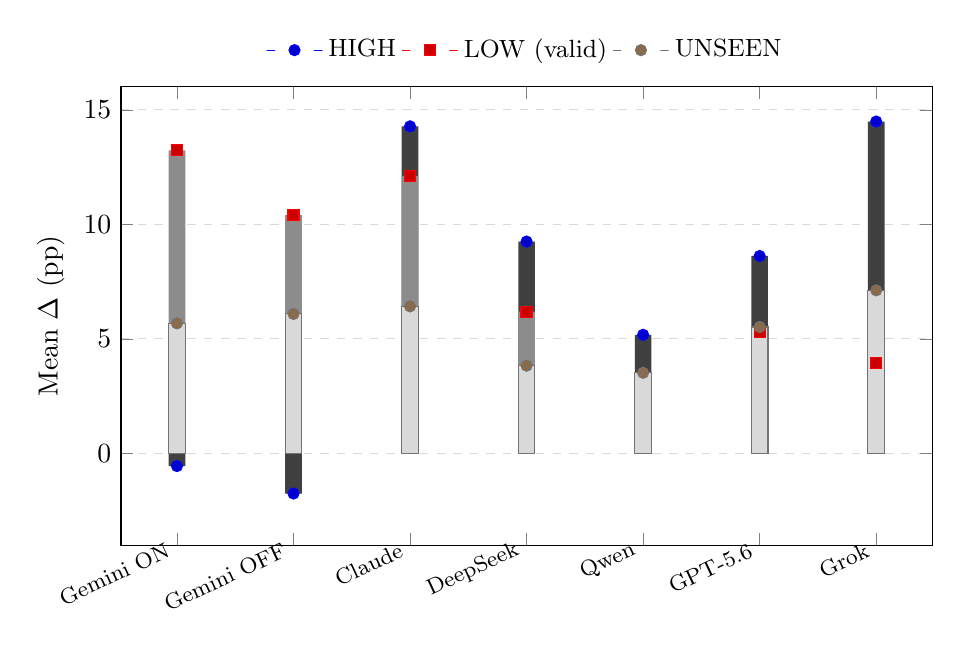
\begin{tikzpicture}
\begin{axis}[
  width=0.98\linewidth,
  height=7.4cm,
  ymajorgrids=true,
  grid style={dashed,gray!30},
  ylabel={Mean $\Delta$ (pp)},
  symbolic x coords={Gemini ON,Gemini OFF,Claude,DeepSeek,Qwen,GPT-5.6,Grok},
  xtick=data,
  x tick label style={rotate=25,anchor=east,font=\footnotesize},
  legend style={at={(0.5,1.03)},anchor=south,legend columns=3,font=\small,draw=none},
  ymin=-4, ymax=16,
  enlarge x limits=0.08,
  bar width=6pt,
]
\addplot+[ybar, fill=black!75, draw=none] coordinates {
  (Gemini ON,-0.55) (Gemini OFF,-1.75) (Claude,14.28) (DeepSeek,9.25)
  (Qwen,5.18) (GPT-5.6,8.62) (Grok,14.49)
};
\addplot+[ybar, fill=black!45, draw=none] coordinates {
  (Gemini ON,13.23) (Gemini OFF,10.40) (Claude,12.11) (DeepSeek,6.19)
  (GPT-5.6,5.31) (Grok,3.95)
};
\addplot+[ybar, fill=black!15, draw=black!55] coordinates {
  (Gemini ON,5.68) (Gemini OFF,6.09) (Claude,6.42) (DeepSeek,3.83)
  (Qwen,3.52) (GPT-5.6,5.52) (Grok,7.12)
};
\legend{HIGH,LOW (valid),UNSEEN}
\end{axis}
\end{tikzpicture}
\caption{Configuration-level mean canonical-coverage $\Delta$ across regimes.
LOW omits Qwen (invalid Direct/Primed model mismatch).
Descriptive only; no inferential intervals.}
\label{fig:configdeltas}
\end{figure}

\begin{figure}[t]
\centering
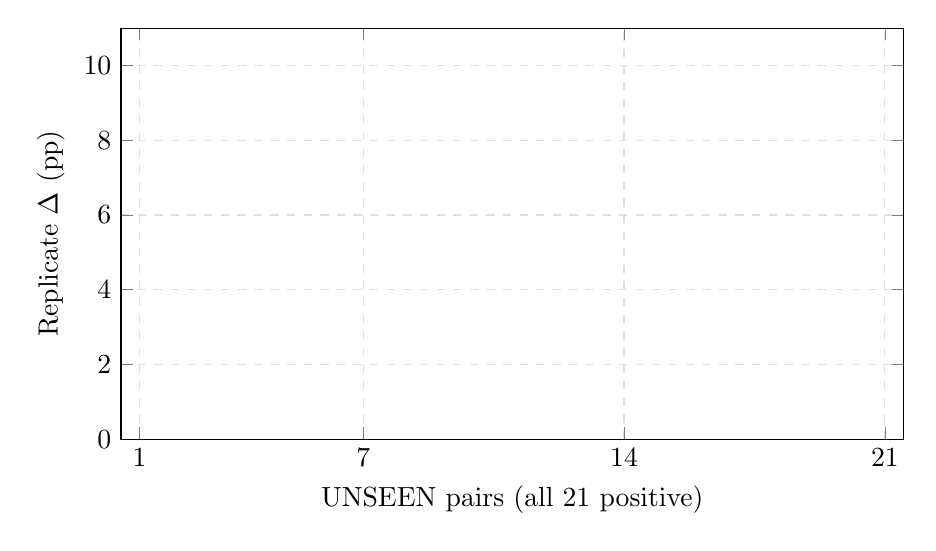
\begin{tikzpicture}
\begin{axis}[
  width=0.95\linewidth,
  height=6.8cm,
  ylabel={Replicate $\Delta$ (pp)},
  xlabel={UNSEEN pairs (all 21 positive)},
  only marks,
  mark size=2.2pt,
  ymin=0, ymax=11,
  xmin=0.5, xmax=21.5,
  xtick={1,7,14,21},
  grid=major,
  grid style={dashed,gray!25},
]
% All 21 UNSEEN replicate deltas from combined analysis (config order)
\addplot[black] coordinates {
  (1,2.12) (2,6.08) (3,8.84)
  (4,7.97) (5,3.96) (6,6.35)
  (7,7.14) (8,5.14) (9,6.96)
  (10,2.91) (11,5.00) (12,3.58)
  (13,3.67) (14,1.27) (15,5.62)
  (16,6.56) (17,7.58) (18,2.43)
  (19,6.02) (20,9.62) (21,5.70)
};
\addplot[gray,dashed,forget plot] coordinates {(0.5,0) (21.5,0)};
\end{axis}
\end{tikzpicture}
\caption{UNSEEN replicate-level paired $\Delta$ values (canonical coverage).
All 21 Direct$\leftrightarrow$Primed pairs are positive.
Points are ordered by configuration (Gemini ON, Gemini OFF, Claude, DeepSeek, Qwen, GPT-5.6 Luna, Grok), three replicates each.
Descriptive display only.}
\label{fig:replicates}
\end{figure}


\subsection{Regime-level reading of the metric}
On HIGH, mean $\Delta$ spans a wide range: from $-1.75$\,pp (Gemini OFF) to $+14.49$\,pp (Grok).
On LOW, valid means are all positive and Gemini becomes strongly positive.
On UNSEEN, means are moderate and uniformly signed at both configuration and replicate levels.
These patterns answer different questions: HIGH shows that priming is not uniformly helpful under the metric even when overlap is high; LOW and UNSEEN show that positive associations are not confined to high-overlap narrative material.

\subsection{Answering RQ1--RQ3 at the metric level}
RQ1: priming is associated with measurable $\Delta$ shifts, but not with a single universal sign on HIGH.
RQ2: on LOW, every \emph{valid} configuration mean $\Delta$ is positive; Gemini means are large ($+13.23$ / $+10.40$\,pp).
RQ3: on UNSEEN, every configuration mean $\Delta$ is positive and every replicate $\Delta$ is positive.
These statements are descriptive coverage observations, not quality or causality claims.


\subsection{Configuration-level commentary (descriptive)}
The following comments restate \Cref{tab:deltas} in prose so that later Discussion can refer to patterns without reintroducing numbers from memory.

\paragraph{Gemini.}
Both Gemini configurations have negative mean $\Delta$ on HIGH ($-0.55$ and $-1.75$\,pp) with mixed replicate signs.
On LOW they become the largest valid positives ($+13.23$ and $+10.40$\,pp), all replicates positive.
On UNSEEN they remain positive ($+5.68$ and $+6.09$\,pp), all replicates positive.
This is the clearest cross-regime reversal in the study.

\paragraph{Claude Sonnet 5.}
Claude is positive in every regime mean and every replicate in the primary tables.
Magnitudes are large on HIGH/LOW and smaller on UNSEEN.
The pattern is persistence with attenuation toward the short technical source, not a sign flip.

\paragraph{DeepSeek Expert ON.}
DeepSeek is likewise persistently positive, with a smooth attenuation sequence $+9.25\rightarrow +6.19\rightarrow +3.83$\,pp.
Among valid configurations, it is one of the clearest monotonic magnitude declines across the three regimes.

\paragraph{Qwen 3.8 Max Fast.}
Qwen contributes valid positive means on HIGH ($+5.18$\,pp, mixed replicates) and UNSEEN ($+3.52$\,pp, all positive).
LOW remains invalid; therefore Qwen cannot enter matched-six summaries.

\paragraph{GPT-5.6 Luna.}
GPT is positive everywhere in the primary means, with relatively stable HIGH replicates and similar LOW/UNSEEN magnitudes.
It is an example of a moderate, persistent association rather than an extreme HIGH-only spike.

\paragraph{Grok 4.5 Fast.}
Grok shows a large HIGH mean ($+14.49$\,pp), a much smaller LOW mean ($+3.95$\,pp) with one negative replicate, and a positive UNSEEN mean ($+7.12$\,pp).
The scientific point is magnitude instability across regimes, not a claim that Grok is ``best'' or ``worst.''
